\documentclass[11pt,a4paper]{report}
\usepackage[textwidth=37em,vmargin=30mm]{geometry}
\usepackage{calc,xunicode,amsmath,amssymb,paralist,enumitem,tabu,booktabs,datetime2,xeCJK,xeCJKfntef,listings}
\usepackage{tocloft,fancyhdr,tcolorbox,xcolor,graphicx,eso-pic,xltxtra,xelatexemoji}

\newcommand{\envyear}[0]{2025}
\newcommand{\envdatestr}[0]{2025-05-15}
\newcommand{\envfinaldir}[0]{webdb/2025/20250515/final}

\usepackage[hidelinks]{hyperref}
\hypersetup{
    colorlinks=false,
    pdfpagemode=FullScreen,
    pdftitle={Web Digest - \envdatestr}
}

\setlength{\cftbeforechapskip}{10pt}
\renewcommand{\cftchapfont}{\rmfamily\bfseries\large\raggedright}
\setlength{\cftbeforesecskip}{2pt}
\renewcommand{\cftsecfont}{\sffamily\small\raggedright}

\setdefaultleftmargin{2em}{2em}{1em}{1em}{1em}{1em}

\usepackage{xeCJK,xeCJKfntef}
\xeCJKsetup{PunctStyle=plain,RubberPunctSkip=false,CJKglue=\strut\hskip 0pt plus 0.1em minus 0.05em,CJKecglue=\strut\hskip 0.22em plus 0.2em}
\XeTeXlinebreaklocale "zh"
\XeTeXlinebreakskip = 0pt


\setmainfont{Brygada 1918}
\setromanfont{Brygada 1918}
\setsansfont{IBM Plex Sans}
\setmonofont{JetBrains Mono NL}
\setCJKmainfont{Noto Serif CJK SC}
\setCJKromanfont{Noto Serif CJK SC}
\setCJKsansfont{Noto Sans CJK SC}
\setCJKmonofont{Noto Sans CJK SC}

\setlength{\parindent}{0pt}
\setlength{\parskip}{8pt}
\linespread{1.15}

\lstset{
	basicstyle=\ttfamily\footnotesize,
	numbersep=5pt,
	backgroundcolor=\color{black!5},
	showspaces=false,
	showstringspaces=false,
	showtabs=false,
	tabsize=2,
	captionpos=b,
	breaklines=true,
	breakatwhitespace=true,
	breakautoindent=true,
	linewidth=\textwidth
}






\newcommand{\coverpic}[2]{
    % argv: itemurl, authorname
    Cover photo by #2~~(\href{#1}{#1})
}
\newcommand{\makeheader}[0]{
    \begin{titlepage}
        % \newgeometry{hmargin=15mm,tmargin=21mm,bmargin=12mm}
        \begin{center}
            
            \rmfamily\scshape
            \fontspec{BaskervilleF}
            \fontspec{Old Standard}
            \fontsize{59pt}{70pt}\selectfont
            WEB\hfill DIGEST
            
            \vfill
            % \vskip 30pt
            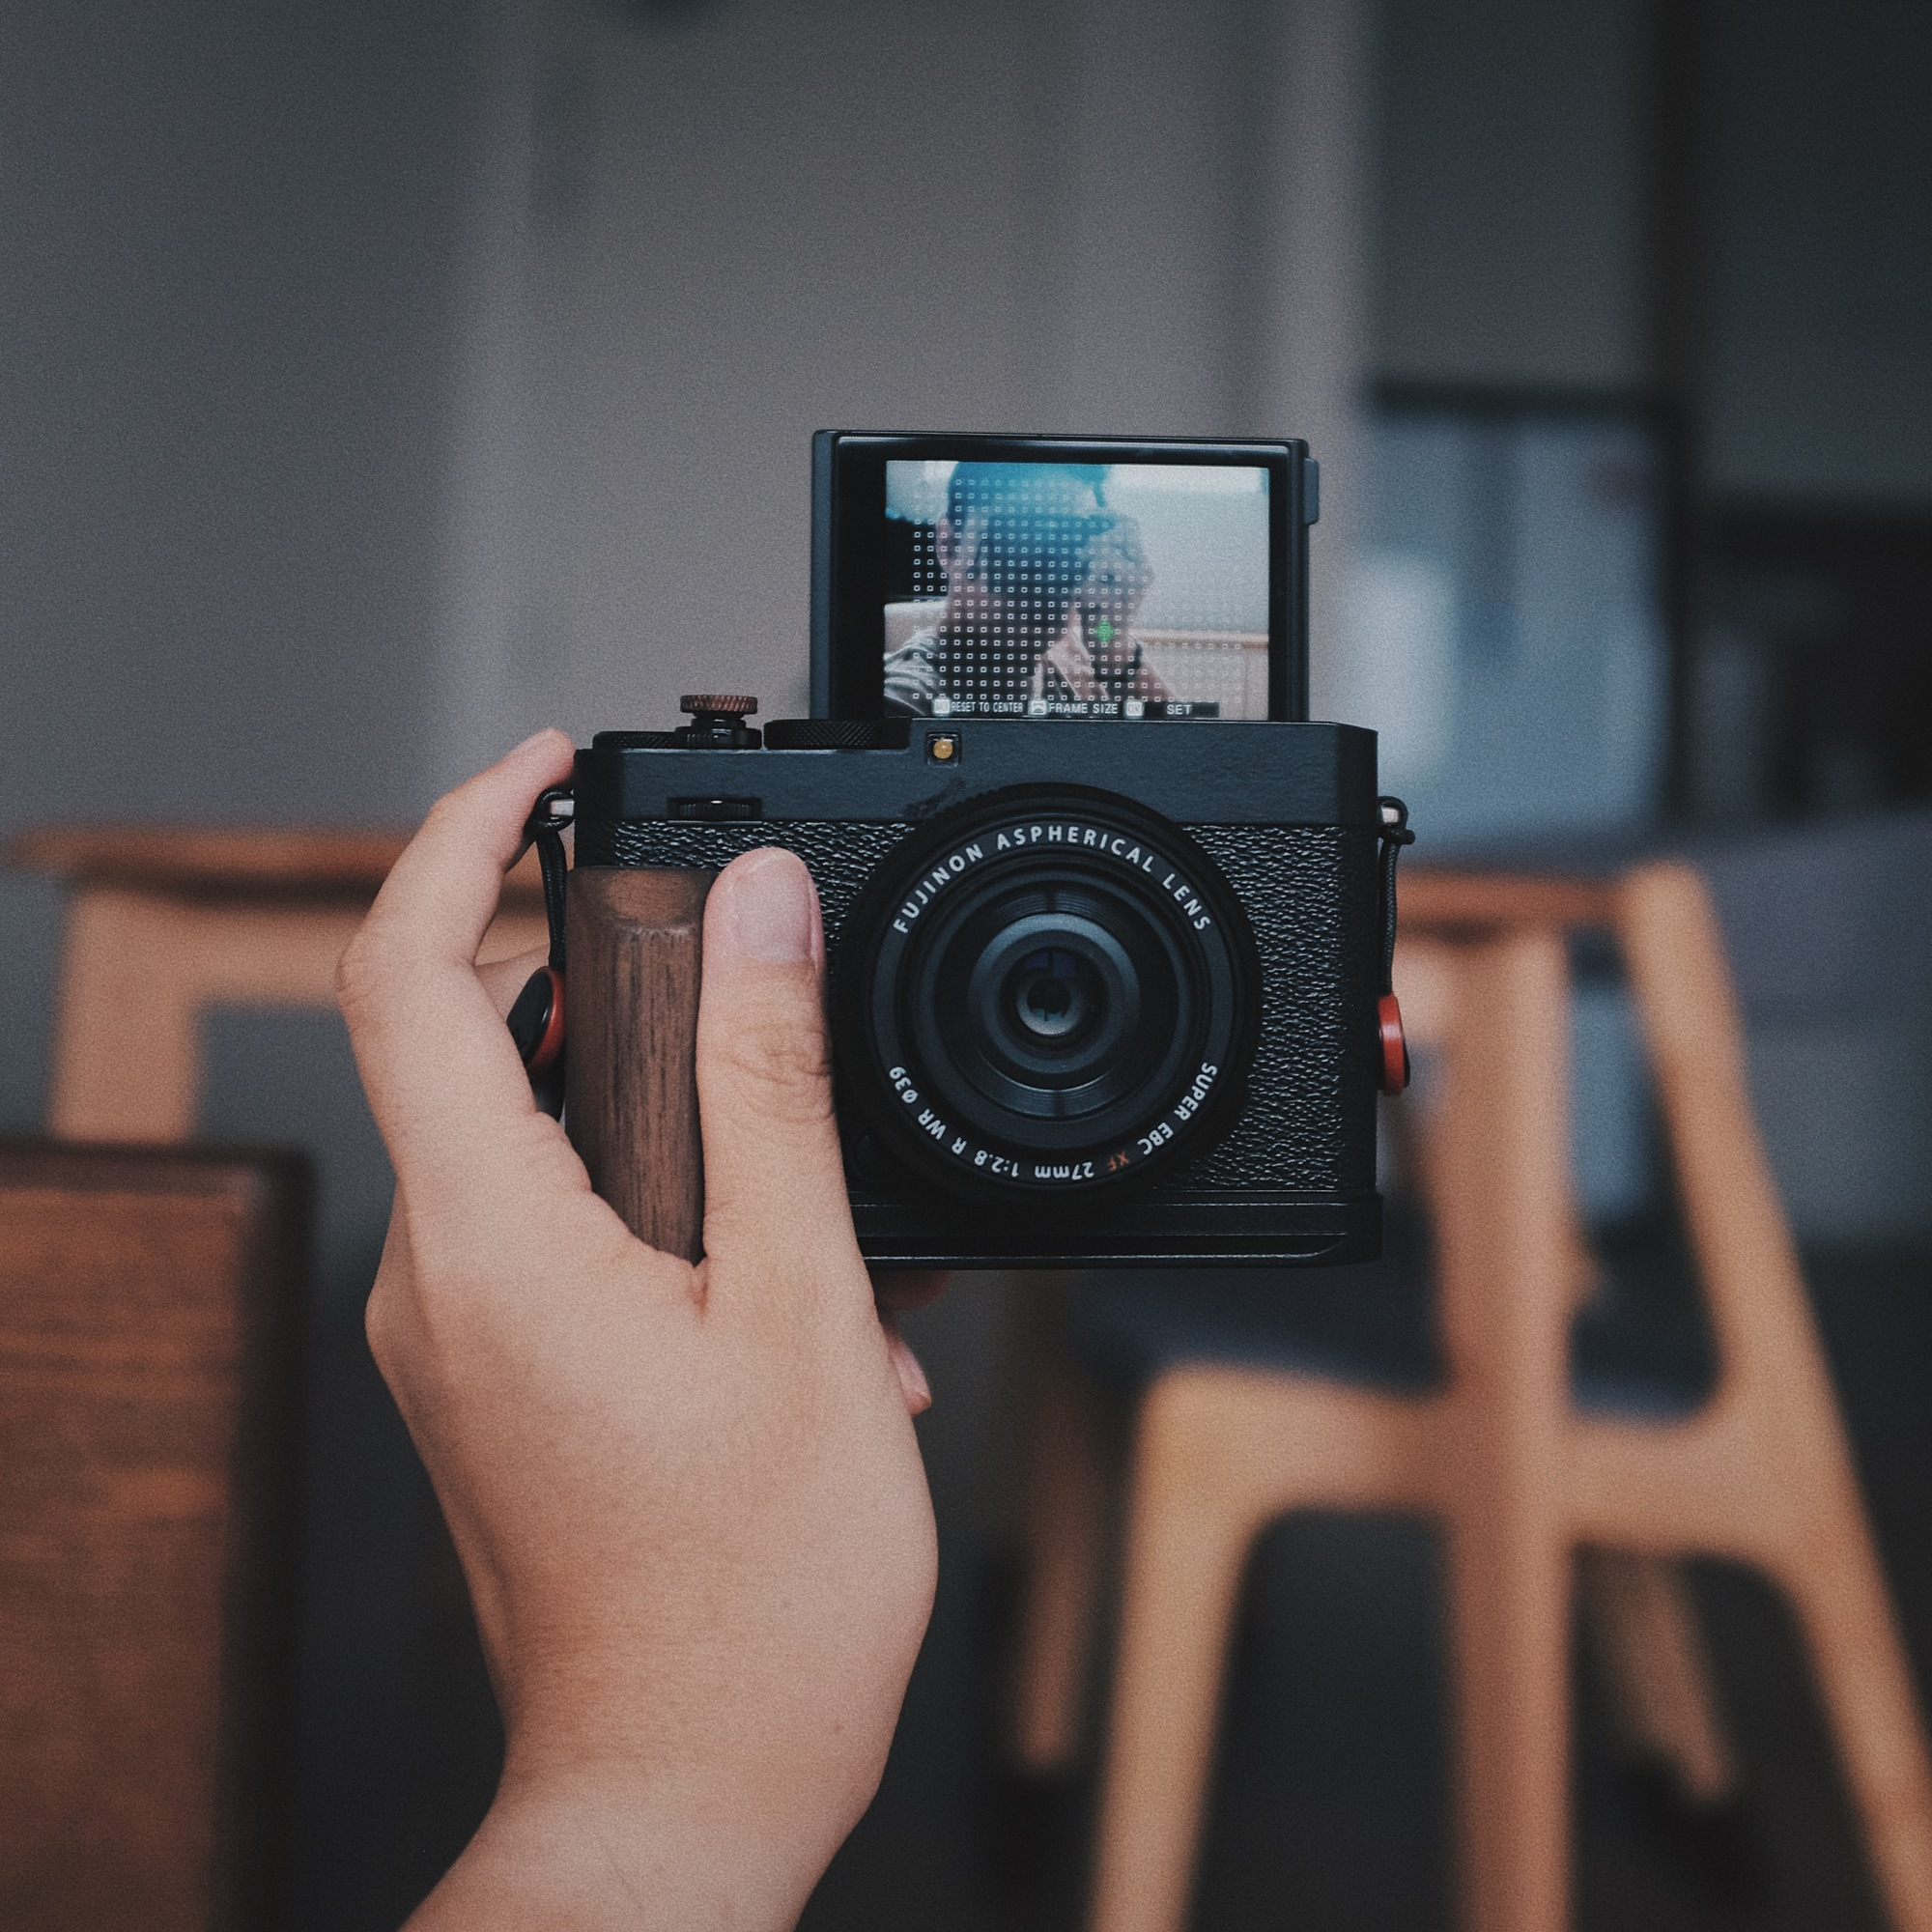
\includegraphics[width=\linewidth]{\envfinaldir/coverpic-prod.jpg}\par
            % \vskip 30pt
            \vfill

            \normalsize\rmfamily\scshape
            \copyright{} The Web Digest Project \hfill\large \envdatestr
        \end{center}
    \end{titlepage}
    % \restoregeometry
}
\newcommand{\simplehref}[1]{%
    \textcolor{blue!80!green}{\href{#1}{#1}}%
}
\renewcommand{\contentsname}{\center\Huge\sffamily\bfseries Contents\par\vskip 20pt}
\newcounter{ipartcounter}
\setcounter{ipartcounter}{0}
\newcommand{\ipart}[1]{
    % \vskip 20pt
    \clearpage
    \stepcounter{ipartcounter}
    \phantomsection
    \addcontentsline{toc}{chapter}{#1}
    % \begin{center}
    %     \Huge
    %     \sffamily\bfseries
    %     #1
    % \end{center}
    % \vskip 20pt plus 7pt
}
\newcounter{ichaptercounter}
\setcounter{ichaptercounter}{0}
\newcommand{\ichapter}[1]{
    % \vskip 20pt
    \clearpage
    \stepcounter{ichaptercounter}
    \phantomsection
    \addcontentsline{toc}{section}{\numberline{\arabic{ichaptercounter}}#1}
    \begin{center}
        \Huge
        \sffamily\bfseries
        #1
    \end{center}
    \vskip 20pt plus 7pt
}
\newcommand{\entrytitlefont}[1]{\subsection*{\raggedright\Large\sffamily\bfseries#1}}
\newcommand{\entryitemGeneric}[2]{
    % argv: title, url
    \parbox{\linewidth}{
        \entrytitlefont{#1}\par\vskip 5pt
        \footnotesize\ttfamily\mdseries
        \simplehref{#2}
    }\vskip 11pt plus 11pt minus 1pt
}
\newcommand{\entryitemGithub}[3]{
    % argv: title, url, desc
    \parbox{\linewidth}{
        \entrytitlefont{#1}\par\vskip 5pt
        \footnotesize\ttfamily\mdseries
        \simplehref{#2}\par\vskip 5pt
        \small\rmfamily\mdseries#3
    }\vskip 11pt plus 11pt minus 1pt
}
\newcommand{\entryitemAp}[3]{
    % argv: title, url, desc
    \parbox{\linewidth}{
        \entrytitlefont{#1}\par\vskip 5pt
        \footnotesize\ttfamily\mdseries
        \simplehref{#2}\par\vskip 5pt
        \small\rmfamily\mdseries#3
    }\vskip 11pt plus 11pt minus 1pt
}
\newcommand{\entryitemHackernews}[3]{
    % argv: title, hnurl, rawurl
    % \parbox{\linewidth}{
    %     \entrytitlefont{#1}\par\vskip 5pt
    %     \footnotesize\ttfamily\mdseries
    %     \simplehref{#3}\par
    %     \textcolor{black!50}{\href{#2}{#2}}
    % }\vskip 11pt plus 11pt minus 1pt
    \begin{minipage}{\linewidth}
            \entrytitlefont{#1}\par\vskip 5pt
            \footnotesize\ttfamily\mdseries
            \simplehref{#3}\par
            \textcolor{black!50}{\href{#2}{#2}}
    \end{minipage}\par\vskip 11pt plus 11pt minus 1pt
}







\begin{document}

\makeheader

\tableofcontents\clearpage




\ipart{Developers}
\ichapter{Hacker News}
\entryitemTwoLinks{Show HN: Muscle-Mem, a behavior cache for AI agents}{https://news.ycombinator.com/item?id=43988381}{https://github.com/pig-dot-dev/muscle-mem}

\entryitemTwoLinks{Perverse incentives of vibe coding}{https://news.ycombinator.com/item?id=43988315}{https://fredbenenson.medium.com/the-perverse-incentives-of-vibe-coding-23efbaf75aee}

\entryitemTwoLinks{Our narrative prison}{https://news.ycombinator.com/item?id=43986424}{https://aeon.co/essays/why-does-every-film-and-tv-series-seem-to-have-the-same-plot}

\entryitemTwoLinks{A server that wasn't meant to exist}{https://news.ycombinator.com/item?id=43985971}{https://it-notes.dragas.net/2025/05/13/the\_server\_that\_wasnt\_meant\_to\_exist/}

\entryitemTwoLinks{Uber to introduce fixed-route shuttles in major US cities}{https://news.ycombinator.com/item?id=43985861}{https://techcrunch.com/2025/05/14/uber-to-introduce-fixed-route-shuttles-in-major-us-cities-other-ways-to-save/}

\entryitemTwoLinks{Show HN: Lumier – Run macOS VMs in a Docker}{https://news.ycombinator.com/item?id=43985624}{https://github.com/trycua/cua/tree/main/libs/lumier}

\entryitemTwoLinks{AlphaEvolve: A Gemini-powered coding agent for designing advanced algorithms}{https://news.ycombinator.com/item?id=43985489}{https://deepmind.google/discover/blog/alphaevolve-a-gemini-powered-coding-agent-for-designing-advanced-algorithms/}

\entryitemTwoLinks{SMS 2FA is not just insecure, it's also hostile to mountain people}{https://news.ycombinator.com/item?id=43984297}{https://blog.stillgreenmoss.net/sms-2fa-is-not-just-insecure-its-also-hostile-to-mountain-people}

\entryitemTwoLinks{U.S. nuclear base hidden under Greenland's ice for decades}{https://news.ycombinator.com/item?id=43984275}{https://www.wsj.com/world/greenland-us-camp-century-nuclear-base-91e8abea}

\entryitemTwoLinks{How the economics of multitenancy work}{https://news.ycombinator.com/item?id=43984097}{https://www.blacksmith.sh/blog/the-economics-of-operating-a-ci-cloud}

\entryitemTwoLinks{The A.I. Radiologist Will Not Be with You Soon}{https://news.ycombinator.com/item?id=43983928}{https://www.nytimes.com/2025/05/14/technology/ai-jobs-radiologists-mayo-clinic.html}

\entryitemTwoLinks{What is HDR, anyway?}{https://news.ycombinator.com/item?id=43983871}{https://www.lux.camera/what-is-hdr/}

\entryitemTwoLinks{E-COM: The \$40M USPS project to send email on paper}{https://news.ycombinator.com/item?id=43983455}{https://buttondown.com/blog/the-e-com-story}

\entryitemTwoLinks{The cryptography behind passkeys}{https://news.ycombinator.com/item?id=43983159}{https://blog.trailofbits.com/2025/05/14/the-cryptography-behind-passkeys/}

\entryitemTwoLinks{Databricks and Neon}{https://news.ycombinator.com/item?id=43982777}{https://www.databricks.com/blog/databricks-neon}

\entryitemTwoLinks{\$20K Bounty Offered for Optimizing Rust Code in Rav1d AV1 Decoder}{https://news.ycombinator.com/item?id=43982238}{https://www.memorysafety.org/blog/rav1d-perf-bounty/}

\entryitemTwoLinks{How to Build a Smartwatch: Picking a Chip}{https://news.ycombinator.com/item?id=43981680}{https://ericmigi.com/blog/how-to-build-a-smartwatch-picking-a-chip/}

\entryitemTwoLinks{Wise refuses to let us access our \$60k AUD}{https://news.ycombinator.com/item?id=43981582}{https://hey.paris/posts/wise/}

\entryitemTwoLinks{The recently lost file upload feature in the Nextcloud app for Android}{https://news.ycombinator.com/item?id=43981170}{https://nextcloud.com/blog/nextcloud-android-file-upload-issue-google/}

\entryitemTwoLinks{Bus stops here: Shanghai lets riders design their own routes}{https://news.ycombinator.com/item?id=43980845}{https://www.sixthtone.com/news/1017072}\ichapter{Phoronix}
\entryitemGeneric{\hskip 0pt{}AMD Ryzen 9 9900 Series Linux Performance Since Launch}{https://www.phoronix.com/review/ryzen-9900-linux-2025}

\entryitemGeneric{\hskip 0pt{}Oracle Talks Up Its Adaptived Daemon For Linux Systems}{https://www.phoronix.com/news/Oracle-Linux-Adaptived}

\entryitemGeneric{\hskip 0pt{}Sovereign Tech Agency Investing In GCC's Fortran Frontend "GFortran"}{https://www.phoronix.com/news/Sovereign-Tech-Agency-GFortran}

\entryitemGeneric{\hskip 0pt{}New Features Approved For Fedora 43}{https://www.phoronix.com/news/Fedora-43-Approves-CMake-4-More}

\entryitemGeneric{\hskip 0pt{}Rustls Server-Side Performance Looking Very Good Compared To OpenSSL}{https://www.phoronix.com/news/Rustls-Server-Side-Beat-OpenSSL}

\entryitemGeneric{\hskip 0pt{}AMD Begins Process Of Preparing The Linux Kernel For Zen 6 CPUs}{https://www.phoronix.com/news/AMD-Zen-6-Linux-Kernel-Start}

\entryitemGeneric{\hskip 0pt{}Oracle Solaris 11.4.81 CBE Released After Three Year Hiatus}{https://www.phoronix.com/news/Oracle-Solaris-11.4.81-CBE}

\entryitemGeneric{\hskip 0pt{}Red Hat Enterprise Linux 10 Reaches GA}{https://www.phoronix.com/news/Red-Hat-RHEL-10-GA}

\entryitemGeneric{\hskip 0pt{}Branch Privilege Injection Vulnerability Disclosed For Intel CPUs}{https://www.phoronix.com/news/Branch-Privilege-Injection}\ichapter{Dribbble}
\entryitemGeneric{\hskip 0pt{}Type Illustration}{https://dribbble.com/shots/26023946-Type-Illustration}

\entryitemGeneric{\hskip 0pt{}UX Logo Icon Concept}{https://dribbble.com/shots/26018312-UX-Logo-Icon-Concept}

\entryitemGeneric{\hskip 0pt{}DropX // Website}{https://dribbble.com/shots/26017012-DropX-Website}

\entryitemGeneric{\hskip 0pt{}@bitcoin website}{https://dribbble.com/shots/26005022--bitcoin-website}

\entryitemGeneric{\hskip 0pt{}Dublo - Logo Design}{https://dribbble.com/shots/26017446-Dublo-Logo-Design}

\entryitemGeneric{\hskip 0pt{}Crypto Portfolio Tracker App}{https://dribbble.com/shots/26017408-Crypto-Portfolio-Tracker-App}

\entryitemGeneric{\hskip 0pt{}Trackwallet}{https://dribbble.com/shots/26013877-Trackwallet}

\entryitemGeneric{\hskip 0pt{}Coffee Brand Redesigns}{https://dribbble.com/shots/26012543-Coffee-Brand-Redesigns}

\entryitemGeneric{\hskip 0pt{}Data Wollet Logo Concept}{https://dribbble.com/shots/26013441-Data-Wollet-Logo-Concept}

\entryitemGeneric{\hskip 0pt{}D\&D stuff}{https://dribbble.com/shots/26011464-D-D-stuff}

\entryitemGeneric{\hskip 0pt{}Branding for AURA — your personal AI assistant}{https://dribbble.com/shots/26010311-Branding-for-AURA-your-personal-AI-assistant}

\entryitemGeneric{\hskip 0pt{}Enfinity Wordmark}{https://dribbble.com/shots/26013368-Enfinity-Wordmark}

\entryitemGeneric{\hskip 0pt{}Finance Website Design}{https://dribbble.com/shots/26008578-Finance-Website-Design}

\entryitemGeneric{\hskip 0pt{}Dataseed®}{https://dribbble.com/shots/25810126-Dataseed}

\entryitemGeneric{\hskip 0pt{}Retro stripes I}{https://dribbble.com/shots/26013911-Retro-stripes-I}

\entryitemGeneric{\hskip 0pt{}LUVI – Wordmark Logo Design}{https://dribbble.com/shots/26006817-LUVI-Wordmark-Logo-Design}

\entryitemGeneric{\hskip 0pt{}ThinkDo on UI8 illustration set}{https://dribbble.com/shots/25995870-ThinkDo-on-UI8-illustration-set}

\entryitemGeneric{\hskip 0pt{}Tweakbird}{https://dribbble.com/shots/26003748-Tweakbird}

\entryitemGeneric{\hskip 0pt{}Seeing Beyond}{https://dribbble.com/shots/26003672-Seeing-Beyond}

\entryitemGeneric{\hskip 0pt{}Logo Roundup > Elegant Vibe}{https://dribbble.com/shots/26000783-Logo-Roundup-Elegant-Vibe}

\entryitemGeneric{\hskip 0pt{}CTRL the Chaos // Dashboard}{https://dribbble.com/shots/25997365-CTRL-the-Chaos-Dashboard}

\entryitemGeneric{\hskip 0pt{}JOUI-yoga for kids}{https://dribbble.com/shots/25997787-JOUI-yoga-for-kids}

\entryitemGeneric{\hskip 0pt{}Meta - Logo Concept}{https://dribbble.com/shots/25998641-Meta-Logo-Concept}

\entryitemGeneric{\hskip 0pt{}Novure - Fashion Online Store e-Commerce Landing Page Animation}{https://dribbble.com/shots/25995753-Novure-Fashion-Online-Store-e-Commerce-Landing-Page-Animation}


\ipart{Developers~~~~(zh-Hans)}
\ichapter{Solidot}
\entryitemGeneric{\hskip 0pt{}微软裁员 3\%}{https://www.solidot.org/story?sid=81284}

\entryitemGeneric{\hskip 0pt{}Telegram 封禁被指洗钱高达 84 亿美元的新币担保}{https://www.solidot.org/story?sid=81283}

\entryitemGeneric{\hskip 0pt{}粘性天然聚合物能清除水中的大多数微塑料}{https://www.solidot.org/story?sid=81282}

\entryitemGeneric{\hskip 0pt{}Google 测试用 AI Mode 取代 I'm Feeling Lucky 按钮}{https://www.solidot.org/story?sid=81281}

\entryitemGeneric{\hskip 0pt{}西部数据投资声称能将数据保存 5000 年的德国公司}{https://www.solidot.org/story?sid=81280}

\entryitemGeneric{\hskip 0pt{}气候危机威胁香蕉}{https://www.solidot.org/story?sid=81279}

\entryitemGeneric{\hskip 0pt{}Firefox 源代码迁移到 GitHub}{https://www.solidot.org/story?sid=81278}

\entryitemGeneric{\hskip 0pt{}猫为什么比狗长寿?}{https://www.solidot.org/story?sid=81277}

\entryitemGeneric{\hskip 0pt{}日产计划裁员两万人}{https://www.solidot.org/story?sid=81276}

\entryitemGeneric{\hskip 0pt{}英伟达据报上调 GPU MSRP 5-15\%}{https://www.solidot.org/story?sid=81275}

\entryitemGeneric{\hskip 0pt{}木星极光的规模和亮度远超地球}{https://www.solidot.org/story?sid=81274}

\entryitemGeneric{\hskip 0pt{}6月11日Showcase 2025 北京-火山引擎专场,热招中}{https://www.solidot.org/story?sid=81272}

\entryitemGeneric{\hskip 0pt{}加密货币公司创始人伪造了自己的死亡}{https://www.solidot.org/story?sid=81270}

\entryitemGeneric{\hskip 0pt{}人人都想要 Chrome}{https://www.solidot.org/story?sid=81269}

\entryitemGeneric{\hskip 0pt{}中美宣布大幅降低关税}{https://www.solidot.org/story?sid=81268}

\entryitemGeneric{\hskip 0pt{}美国 25 个大城市在下沉}{https://www.solidot.org/story?sid=81267}

\entryitemGeneric{\hskip 0pt{}参宿四超新星爆发是否会毁灭地球?}{https://www.solidot.org/story?sid=81266}

\entryitemGeneric{\hskip 0pt{}基因编辑让蜘蛛吐彩丝}{https://www.solidot.org/story?sid=81265}

\entryitemGeneric{\hskip 0pt{}deepin 社区表示将改进安全响应和修复安全问题}{https://www.solidot.org/story?sid=81264}

\entryitemGeneric{\hskip 0pt{}美国版权局不认为使用版权材料训练 AI 是合理使用,特朗普随即解雇了局长}{https://www.solidot.org/story?sid=81263}\ichapter{V2EX}
\entryitemGeneric{\hskip 0pt{}[NAS] Apple TV 上的 Jellyfin 客户端选择?}{https://www.v2ex.com/t/1131841}

\entryitemGeneric{\hskip 0pt{}[Flutter] 应用未声明 QUERY\_ALL\_PACKAGES 权限却报错,是 firebase 导致的吗?}{https://www.v2ex.com/t/1131839}

\entryitemGeneric{\hskip 0pt{}[创业组队] 开发者诚征市场推广合伙人}{https://www.v2ex.com/t/1131838}

\entryitemGeneric{\hskip 0pt{}[优惠信息] windsurf pro 免费一个月}{https://www.v2ex.com/t/1131837}

\entryitemGeneric{\hskip 0pt{}[北京] 北京哪里有可以租用的影音馆?}{https://www.v2ex.com/t/1131836}

\entryitemGeneric{\hskip 0pt{}[问与答] 大家平时都是怎么管理信用卡账单的}{https://www.v2ex.com/t/1131835}

\entryitemGeneric{\hskip 0pt{}[问与答] v0 收费方式变了 好贵了,有没有便宜的方案.}{https://www.v2ex.com/t/1131834}

\entryitemGeneric{\hskip 0pt{}[酷工作] [广州][外资银行]Senior Container Engineer}{https://www.v2ex.com/t/1131833}

\entryitemGeneric{\hskip 0pt{}[问与答] 阿里系的软件真的是不是都是这么恶心啊}{https://www.v2ex.com/t/1131831}

\entryitemGeneric{\hskip 0pt{}[梦] 早睡是为了在梦里待久一点}{https://www.v2ex.com/t/1131830}

\entryitemGeneric{\hskip 0pt{}[职场话题] 京东开发岗位的职级有什么用吗}{https://www.v2ex.com/t/1131829}

\entryitemGeneric{\hskip 0pt{}[Google] 精通 google 优化的来}{https://www.v2ex.com/t/1131828}

\entryitemGeneric{\hskip 0pt{}[程序员] 脚本化 VS 可视化节点,谁将更胜一筹?}{https://www.v2ex.com/t/1131827}

\entryitemGeneric{\hskip 0pt{}[问与答] 外卖自动抢单的想法可行不}{https://www.v2ex.com/t/1131826}

\entryitemGeneric{\hskip 0pt{}[NAS] [2025 年推荐] 黑群晖/飞牛整机 NAS/自组 NAS}{https://www.v2ex.com/t/1131824}

\entryitemGeneric{\hskip 0pt{}[商业模式] 创业想法}{https://www.v2ex.com/t/1131823}

\entryitemGeneric{\hskip 0pt{}[投资] 这下是真的塌了,黄金贴破 740 了...}{https://www.v2ex.com/t/1131822}

\entryitemGeneric{\hskip 0pt{}[职场话题] 后知后觉,自己已经被淘汰了}{https://www.v2ex.com/t/1131820}

\entryitemGeneric{\hskip 0pt{}[DNS] 分享一个付费的 DOH,大家可以试试}{https://www.v2ex.com/t/1131818}

\entryitemGeneric{\hskip 0pt{}[分享创造] 发现很多人还不知道这个网站!}{https://www.v2ex.com/t/1131816}

\entryitemGeneric{\hskip 0pt{}[生活] 按摩椅购买的性价比高吗}{https://www.v2ex.com/t/1131815}

\entryitemGeneric{\hskip 0pt{}[程序员] gemini\_2.5\_pro\_preview\_0506 让我头皮发麻}{https://www.v2ex.com/t/1131814}

\entryitemGeneric{\hskip 0pt{}[MacBook Air] 各位 v 友们问个事情}{https://www.v2ex.com/t/1131813}

\entryitemGeneric{\hskip 0pt{}[分享创造] Overlay 免费 AI 助手 v0.6.0}{https://www.v2ex.com/t/1131809}

\entryitemGeneric{\hskip 0pt{}[分享发现] 自己撸了一个 ai 生成线稿的网站,线稿素材天花板}{https://www.v2ex.com/t/1131808}

\entryitemGeneric{\hskip 0pt{}[投资] 今晚黄金大跌,我的空单平仓了离场了}{https://www.v2ex.com/t/1131806}

\entryitemGeneric{\hskip 0pt{}[汽车] 各位老哥求帮忙,方程豹和理想选哪个?}{https://www.v2ex.com/t/1131805}

\entryitemGeneric{\hskip 0pt{}[职场话题] 35 岁中年, offer 二选一,求各位大佬帮忙参考参考}{https://www.v2ex.com/t/1131804}

\entryitemGeneric{\hskip 0pt{}[VPS] 搬瓦工自建的梯子用不了 TG 电报}{https://www.v2ex.com/t/1131803}

\entryitemGeneric{\hskip 0pt{}[问与答] ios 上面 怎么方便的用上双拼 [智能 ABC] 方案?}{https://www.v2ex.com/t/1131802}

\entryitemGeneric{\hskip 0pt{}[程序员] 前端 service worker 代码, 有测试用例的必要不}{https://www.v2ex.com/t/1131801}

\entryitemGeneric{\hskip 0pt{}[程序员] 如何申请 AI 模型的 API?}{https://www.v2ex.com/t/1131800}

\entryitemGeneric{\hskip 0pt{}[分享创造] [小项目] 整理 Apple Siri 隐私和解案信息,做了个查询小站}{https://www.v2ex.com/t/1131799}

\entryitemGeneric{\hskip 0pt{}[程序员] 节点总数固定,如何用最少的通信轮数得到共识的不可预测的随机数?}{https://www.v2ex.com/t/1131798}

\entryitemGeneric{\hskip 0pt{}[问与答] pixel 新手机,是否仍然提供相册无限备份?}{https://www.v2ex.com/t/1131797}

\entryitemGeneric{\hskip 0pt{}[Apple] iOS18.5 国区 Apple ID (非国行 iPhone )也能有 Apple intelligence}{https://www.v2ex.com/t/1131796}

\entryitemGeneric{\hskip 0pt{}[酷工作] 上海游戏厂多个 QA 和后端 HC! T0 员工福利待遇~}{https://www.v2ex.com/t/1131795}

\entryitemGeneric{\hskip 0pt{}[问与答] 有没有能否比较准确识别印度口音/英国口音的语音转文字的软件?}{https://www.v2ex.com/t/1131794}

\entryitemGeneric{\hskip 0pt{}[分享创造] 错过热点,刚上线的网站就要下线了吗?}{https://www.v2ex.com/t/1131793}

\entryitemGeneric{\hskip 0pt{}[游戏] 安卓有没有单机三国策略游戏}{https://www.v2ex.com/t/1131791}

\entryitemGeneric{\hskip 0pt{}[职场话题] 外包转正式工,需要哪些证明,以便以后证明在同一家单位工作}{https://www.v2ex.com/t/1131790}

\entryitemGeneric{\hskip 0pt{}[剧集] 整理一下这十几年追过的剧集}{https://www.v2ex.com/t/1131789}

\entryitemGeneric{\hskip 0pt{}[分享发现] 字节,吃香不要太难看}{https://www.v2ex.com/t/1131788}

\entryitemGeneric{\hskip 0pt{}[问与答] 求个 macOS App 可以在输入框快速翻译的小工具}{https://www.v2ex.com/t/1131787}

\entryitemGeneric{\hskip 0pt{}[服务器] 小主机还是 macmini m4?}{https://www.v2ex.com/t/1131786}

\entryitemGeneric{\hskip 0pt{}[Apple] Macos 15.3.1 suggestd 进程高 cpu 占用}{https://www.v2ex.com/t/1131785}

\entryitemGeneric{\hskip 0pt{}[求职] 七年经验实施交付工程师找工作, base 上海}{https://www.v2ex.com/t/1131784}

\entryitemGeneric{\hskip 0pt{}[分享发现] 自媒体时代,我终究是踏出了第一步}{https://www.v2ex.com/t/1131783}

\entryitemGeneric{\hskip 0pt{}[问与答] 如何查看别人用我的电脑的 chrome 干了什么}{https://www.v2ex.com/t/1131781}

\entryitemGeneric{\hskip 0pt{}[全球工单系统] 阿里云杭州负载均衡炸了}{https://www.v2ex.com/t/1131780}


\ipart{Generic News}
\ichapter{联合早报}
\entryitemWithDescription{黎康:魔都的B面}{https://www.zaobao.com/news/china/story20250426-6241474}{``确实这几年上海的城市公共建设很好,但你有没有去看过一些老旧小区的环境?小区里电线横飞,绿化基本毫无规划;进入楼道,你会感觉回到20年前\ldots\ldots'' 上一篇``早点------沪上闲语''发表后,收到一封读者来信。这位上海市民告诉我,在装点城市门面的郁金香背后,如果走进上海的老旧小区,会看到这座城市的另一面……}

\entryitemWithDescription{新闻人间:从``不懂球的胖子''到改革推手——刘国梁}{https://www.zaobao.com/news/china/story20250426-6238850}{中国乒乓球协会星期三(4月23日)突然宣布,刘国梁主动辞去主席一职。这一消息迅速引发体坛热议,有球迷为他的离开感到惋惜,也有体育评论员开始审视他在任期内的功与过。 刘国梁自2018年起担任乒协主席,如今在第二任期尚未结束之际中途请辞,外界难免有诸多猜测。星期三当天,他以主席身份在乒协会议上作最后一次发言时,几度哽咽,甚至当场落泪。 他在记者会上透露,早在去年巴黎奥运会结束后,便已向上级表达了去意……}

\entryitemWithDescription{中国据报考虑暂停加征部分美国产品125\%关税}{https://www.zaobao.com/news/china/story20250425-6245926}{中国政府据报考虑暂停对部分美国进口产品加征125\%的关税,受访学者认为此举主要考虑中国企业的生存需要,与中美是否开启贸易谈判无关。 据彭博社引述知情人士报道,中国政府正考虑取消对美国的医疗设备,以及乙烷等工业化学品加征的报复性关税。中国是全球最大的塑料制造国,但部分工厂依赖从美国进口的乙烷。中国医院也需要美国生产的磁共振成像和超声仪器等医疗设备。 知情人士称,飞机租赁也可能豁免关税……}

\entryitemWithDescription{中国美国商会白皮书:五分之一美企不再视中国为优先投资地}{https://www.zaobao.com/news/china/story20250425-6245113}{中国美国商会的调查显示,五分之一的在华美国企业不再将中国列为优先的投资目的地。 该商会星期五(4月25日)发布由100余名中国美国商会会员企业代表共同撰写的2025年《美国企业在中国白皮书》。 白皮书指出,中美两国关系日益紧张,已连续五年成为在华美资企业面临的首要商业挑战,超过了合规风险和来自中国企业的竞争压力……}

\entryitemWithDescription{中国发布生态调查报告 称菲律宾捕捞现场发现人为弃置物}{https://www.zaobao.com/news/china/story20250425-6244616}{(北京讯)中国多家自然生态机构星期五(4月25日)联合公布一份调查报告,评估铁线礁、牛轭礁珊瑚礁的生态系统状况,称菲律宾所谓``中国在铁线礁倾倒珊瑚碎屑等言论''毫无科学和事实依据。 中国自然资源部微信公号分别发表了这份题为《铁线礁、牛轭礁珊瑚礁生态系统调查报告》的中英文版本,参与编制的机构包括中国自然资源部南海发展研究院、南海生态中心等……}

\entryitemWithDescription{香港公共场所明年起设更多禁烟区 违例罚款提高一倍}{https://www.zaobao.com/news/china/story20250425-6245064}{为了进一步降低吸烟率,香港特区政府将由明年起在更多公共场所设立禁烟区,并把违例吸烟的罚款金额提高一倍至3000港元(508新元)。 相关条例草案星期五(4月25日)刊宪,列明从明年元旦起,禁止在等候公共交通工具、等候进入电影院、医院、公众游乐场地、体育场等地方的划定范围吸烟。违者罚款由1500港元倍增至3000港元……}

\entryitemWithDescription{两韩国顶尖半导体专家 退休后被中国高校任用}{https://www.zaobao.com/news/china/story20250425-6244895}{(首尔讯)中国正通过从海外引进顶尖人才,与美国争夺高科技主导权。韩国两名``国宝级''顶尖专家退休后在本国受到冷落,未能找到合适研究职位,目前已被中国高等学府任用。 据韩国《中央日报》报道,韩国知名碳纳米管专家李永熙去年11月正式受聘于湖北工业大学半导体与量子研究所……}

\entryitemWithDescription{美国传降对陆关税又强化对台论述 分析:谈判或拿台湾当筹码}{https://www.zaobao.com/news/china/story20250425-6244227}{华盛顿释出降低对华关税信号、寻求谈判之际,美国星期三(4月23日)首次在联合国安理会批评北京误用联大2758号决议;更在同一天派遣军舰穿越台湾海峡。受访学者分析,这些作为现阶段暂与关税战没有直接关联,但不排除美国总统特朗普接下来可能利用台湾问题作为对华谈判筹码。 特朗普本周透露考虑大幅度降低对华关税,希望与中国达成``公平的协议'',同时又声称美国每天都同中国直接联系……}

\entryitemWithDescription{韩咏红:特朗普关税从``解放日''走到``妥协日''了?}{https://www.zaobao.com/news/china/story20250425-6240846}{美国总统特朗普在4月2日宣布对等关税政策,短短20天后,特朗普的高姿态已难以为继。特朗普在4月9日就已调整过一次战术,暂缓对其他国家课征对等关税,集中火力单挑中国;而今,特朗普恐怕又要眨眼了,对中国商品课征的145\%关税也可能显著下调。 特朗普近日罕见地对中国伸出橄榄枝,表示考虑大幅度降低对华关税,显露出急于与中国达成协议。但中国偏是表现得不着急……}

\entryitemWithDescription{学者:中国以2+2机制拉拢东南亚国家抗衡美国}{https://www.zaobao.com/news/china/story20250424-6240690}{受访学者分析,在中美关系因贸易战而全面恶化的大背景下,中国正以``外交、国防2+2对话机制''为新抓手,积极拉拢亚细安成员国,以抗衡美国在本区域的影响力,预计中国接下来将推动与更多区域国家建立2+2机制。 中国和印度尼西亚星期一(4月21日)在北京举行外长、防长对话机制下的首次部长级会议,两国在2023年就建立2+2对话机制。中国官方称,这是中国在全球建立的首个部长级2+2机制……}

\entryitemWithDescription{中埃空军首次联训 学者:中国初步具备向中东快速战略投送能力}{https://www.zaobao.com/news/china/story20250424-6240357}{中国空军上周派出多架战斗机、预警机、运输机与空中加油机前往埃及,进行两军首次联训。这是中国空军首次以完整作战体系进行跨洲机动。 受访学者认为,这是中国空军现代化进程的里程碑,有助于发展长途奔袭的技战术;这也标志着中国初步具备向中东进行快速战略投送的能力。 据中国国防部消息,中国与埃及两国空军于4月中旬至5月上旬,在埃及空军基地组织代号为``文明之鹰-2025''的联合训练……}

\entryitemWithDescription{台湾收紧民众申领大陆证照规定 持大陆定居证也将被撤销台湾身份}{https://www.zaobao.com/news/china/story20250424-6239789}{(台北综合讯)台湾再度收紧民众申领中国大陆证照的规定,持有大陆定居证的台湾民众也触犯相关法令,将丧失台湾身份。 综合《旺报》与《联合报》报道,台湾行政院公报显示,陆委会近日对《两岸条例》当中规定发布解释函令称,为确保两岸人员单一身份制度,两岸条例规定台湾人民不得在大陆地区``设有户籍'',或领用大陆地区护照,否则将丧失台湾身份……}

\entryitemWithDescription{神舟二十号成功发射 航天员将开展中国首次涡虫空间再生实验}{https://www.zaobao.com/news/china/story20250424-6239950}{(北京综合讯)中国星期四(4月24日)成功发射神舟二十号载人飞船。三名航天员将在空间站驻留约六个月,并开展中国首次涡虫空间再生实验。 综合新华社、央视新闻和《中国青年报》报道,搭载神舟二十号的长征二号F遥二十运载火箭,星期四下午5时17分在甘肃酒泉卫星发射中心点火发射。约10分钟后,神舟二十号与火箭成功分离,进入预定轨道……}

\entryitemWithDescription{台大罢免升温 朝野对抗加剧}{https://www.zaobao.com/news/china/story20250424-6240062}{台湾两大在野党将携手举办大型造势活动,抗议政府利用司法整肃异己,进行大罢免。兼任民进党主席的总统赖清德则公开肯定公民团体罢免在野党立委的行动影片,检调也持续搜索在野国民党宜兰县党部,朝野对抗情势正逐步升温……}

\entryitemWithDescription{美国国会罕见动用传唤权 调查中国三电信巨头}{https://www.zaobao.com/news/china/story20250424-6239456}{(纽约路透电)美国众议院中国问题特别委员会星期三(4月23日)罕见地动用传唤权,调查中国三大电信公司涉嫌支持中国军方和政府的行为。 据路透社报道,中国移动、中国电信和中国联通三家中国电信巨头收到该委员会的传唤通知,须回答他们是否可通过在美开展的云服务和互联网业务获取美国数据的问题。 美国两党议员持续对被指由中国主导的网络攻击事件表示担忧……}

\entryitemWithDescription{浙江一小学门外发生汽车冲撞人群事件}{https://www.zaobao.com/news/china/story20250424-6238514}{(香港综合讯)中国再发生校园伤人事件,浙江金华一所小学门外星期二(4月22日)放学时有汽车冲撞人群,伤亡人数不明。官方在事发两日后仍未发布通报,中国社媒上的相关信息均被删除。 综合《明报》《南华早报》和网媒``香港01''报道,这起事件发生在金华市苏孟乡中心小学门口,时间是星期二傍晚5时45分左右,正值放学时间。附近商户披露,有多名学生被撞……}

\entryitemWithDescription{学者:关税战伤敌一千自损八百 中美终将找到共处之道}{https://www.zaobao.com/news/china/story20250424-6238821}{美国总统特朗普祭出对等关税将届满一个月,如今传出可能降低对华关税,定居美国的资深华人学者赵全胜指出,中美领导阶层有一批人长期相信对方马上要垮台,但关税战让双方意识到,这无疑是``伤敌一千,自损八百'',因此迟早会找到共处之道。 特朗普4月2日宣布全面实施对等关税,随后在9日紧急暂缓90天,让各国争取与美国谈判的时间与空间,唯独对中国不断加码;北京也不甘示弱,提出相应反制……}

\entryitemWithDescription{打击电诈犯罪扩至纵深地带 缅甸向中国移交920余名嫌犯}{https://www.zaobao.com/news/china/story20250424-6238307}{(北京综合讯)中国与缅甸加大打击电信网络诈骗犯罪合作力度,两国最近一个月的合作执法行动,已从缅北地区扩大到当阳、勐休等缅甸纵深地带。 中国公安部官网星期三(4月23日)通报,缅甸执法部门近日将在当地抓获的920余名中国籍涉诈犯罪嫌疑人,通过云南西双版纳打洛口岸全部移交中国警方。 通报称,缅北电诈犯罪集团遭受重创,但部分涉诈人员为逃避打击,向当阳、勐休等纵深地带转移藏匿,继续实施跨境电诈……}

\entryitemWithDescription{沈泽玮:魔幻山城的中国式现代化演绎}{https://www.zaobao.com/news/china/story20250424-6234868}{时隔12年因工作再访重庆,春夏交替之际迎来烈日当空,与当年冬季旅游行走于山城迷雾的印象截然不同。 5000架无人机灯光秀,既展现科技力量也打造视觉盛宴;科企创始人讲述营商环境不断优化;村委会主任手捧涪陵榨菜分享东方酱腌菜``走出去''成果;火车司机传递通关速度如何带动互联互通跨境贸易;公安局交巡警总队科研处综合科科长讲述数字化赋能超大城市治理;社区党委书记分享中国特色``民主村''的前身今世……}

\entryitemWithDescription{中国网购平台将全面取消``仅退款''}{https://www.zaobao.com/news/china/story20250423-6234242}{在中国官方整治``内卷式竞争''的背景下,中国电商平台将全面取消``仅退款''选项。受访学者认为,此举有助行业回归良性竞争,是对电商市场的一次纠偏。 据《北京商报》报道,拼多多、淘宝、抖音、快手、京东等多个中国电商平台,星期二(4月22日)修改有关``仅退款''的相关条款,消费者申请``退款不退货'',将由商家自主处理……}

\entryitemWithDescription{3月人民币跨境收付占比刷新历史纪录}{https://www.zaobao.com/news/china/story20250423-6233857}{(华盛顿彭博电)随着美元的全球吸引力减弱、中美贸易紧张局势上升,3月中国投资者和贸易公司在国际结算中对人民币的使用大幅增加,创下历史纪录。 彭博社基于中国国家外汇管理局星期二(4月22日)公布的数据计算,3月中国大陆境内个人和机构的跨境业务中,人民币使用占比达 54.3\%,总额7249亿美元(9502亿新元)……}






\clearpage
\leavevmode\vfill
\footnotesize

Copyright \copyright{} 2023-2025 Neruthes and other contributors.

This document is published with CC BY-NC-ND 4.0 license.

The entries listed in this newsletter may be copyrighted by their respective creators.

This newsletter is generated by the Web Digest project.

The newsletters are also delivered via Telegram channel \CJKunderline{\href{https://t.me/webdigestchannel}{https://t.me/webdigestchannel}}.\\
RSS feed is available at \CJKunderline{\href{https://webdigest.pages.dev/rss.xml}{https://webdigest.pages.dev/rss.xml}}.

This newsletter is available in PDF at
\CJKunderline{\href{https://webdigest.pages.dev/}{https://webdigest.pages.dev/}}.

The source code being used to generate this newsletter is available at\\
\CJKunderline{\href{https://github.com/neruthes/webdigest}{https://github.com/neruthes/webdigest}}.

This newsletter is also available in
\CJKunderline{\href{http://webdigest.pages.dev/readhtml/\envyear/WebDigest-20250515.html}{HTML}} and
\CJKunderline{\href{https://github.com/neruthes/webdigest/blob/master/markdown/\envyear/WebDigest-20250515.md}{Markdown}}.


\coverpic{https://unsplash.com/photos/nighttime-view-of-a-vibrant-city-street-kgzcovItVt8}{mos design}


\end{document}
